\chapter{Evaluation}
In this chapter, we analyze the performance impact of the IOMMU, directly comparing it to the physical address approach. To compare both approaches fairly, we allocate and map the memory upfront. The focus lies on the IOMMU itself and how it performs. All performance tests use legacy VFIO instead of IOMMUFD as it currently remains the widely supported way of using the IOMMU.

\section{Setup}
We use two systems to benchmark the driver's performance.
Both systems run Ubuntu 23.10 with Linux kernel version 6.5.0-42 and are NUMA systems with two nodes each. We stick to NUMA locality, ensuring that the tested processes access memory from their nearest available memory node to improve performance.

\begin{table}[H]
  \centering
  \begin{tabular}{lllrll}
    \textbf{CPU}                          & \textbf{Memory}                         & \textbf{NVMe}                         & \textbf{Capacity}                       & \textbf{Count}   \\
    \toprule

    \multirow{2}{*}{Intel Xeon E5-2660v2} & \multirow{2}{*}{\qty{251}{\gibi\byte}}  & \multirow{2}{*}{Samsung Evo 970 Plus} & \multirow{2}{*}{\qty{1}{\tera\byte}}    &
    \multirow{2}{*}{1}                                                                                                                                                                   \\
                                          &                                         &                                       &                                         &                & \\ \hline

    \multirow{2}{*}{AMD EPYC 7713}        & \multirow{2}{*}{\qty{1007}{\gibi\byte}} & \multirow{2}{*}{Samsung PM9A3}        & \multirow{2}{*}{\qty{1.92}{\tera\byte}} &
    \multirow{2}{*}{8}                                                                                                                                                                   \\
                                          &                                         &                                       &                                         &                & \\
    \bottomrule
  \end{tabular}

  \caption{Specifications of systems used in performance testing}
  \label{tab:servers}
\end{table}

\begin{table}[H]
  \centering
  \begin{tabular}{llrrrr}
    \multirow{2}{*}{\textbf{CPU}} & \multirow{2}{*}{\textbf{Clock}} & \multirow{2}{*}{\textbf{Cores}} & \multirow{2}{*}{\textbf{Virtualization}} & \multirow{2}{*}{\textbf{Year}}
    \\
                                  &                                 &                                 &                                          &                                \\
    \toprule

    Intel Xeon E5-2660v2          & \qty{2.2}{\giga\Hz}             & 10                              & VT-d                                     & 2012                           \\
    AMD EPYC 7713                 & \qty{2.0}{\giga\Hz}             & 64                              & AMD-V                                    & 2021                           \\

    \bottomrule
  \end{tabular}

  \caption{CPUs of the systems}
  \label{tab:cpus}
\end{table}

\begin{table}[H]
  \centering
  \begin{tabular}{lrrll}
    \multirow{2}{*}{\textbf{NVMe}} & \textbf{Maximum}     & \textbf{Maximum}    & \multirow{2}{*}{\textbf{Turbowrite}} & \multirow{2}{*}{\textbf{Usage}} \\
                                   & \textbf{Queue Count} & \textbf{Queue Size} &                                      &                                 \\
    \toprule

    Samsung Evo 970 Plus           & 128                  & 16384               & Yes                                  & Consumer                        \\
    Samsung PM9A3                  & 128                  & 16384               & No                                   & Enterprise                      \\

    \bottomrule
  \end{tabular}

  \caption{NVMe(s) of the systems}
  \label{tab:nvmes}
\end{table}

Despite the NVMe specification's maximum capability of 65536 I/O queues, our SSDs support a more reasonable amount of 128 I/O queues, which seems to be typical for modern SSDs.
Turbowrite is a Samsung technology that drastically speeds up write latencies in the so-called "Turbowrite" buffer with the size of \qty{42}{\giga\byte} of the NVMe, as shown in \cite{vroom}. All NVMe SSDs used were formatted to 512-byte blocks.

We use one thread per 1 I/O queue in our multithreaded tests.
All writes are performed on an empty SSD to avoid overhead through garbage collection on the NVMe. As the NVMe can optimize reads on an empty SSD, all reads will be performed on a full SSD. We exclusively use random writes/reads for the tests, as the NVMe can drastically optimize sequential requests, which can lead to altered results.
Unless stated otherwise, we configure the submission and completion queue length to the maximum amount supported by the NVMes.
Additionally, all standard tests are run with the \texttt{iommu.strict=1} kernel parameter. When this parameter is set, the IOMMU invalidates the complete IOTLB when an unmapping occurs. As we unmap IOVAs in between tests, this ensures that the IOTLB is flushed before each test.

\section{Results}
For the following performance tests, we will compare the latencies and throughput of vroom without the IOMMU and with the IOMMU, both utilizing \qty{2}{\mebi\byte} pages. All latency and throughput tests are run with a \qty{1}{\gibi\byte} buffer in memory. For \qty{2}{\mebi\byte} pages, this equates to 512 pages being accessed. We use a unit size of \qty{4}{\kibi\byte}, i.e., each I/O operation reads/writes \qty{4}{\kibi\byte} to the the NVMe.

\subsection{Latencies}
All latency performance measurements are done singlethreaded with queue depth 1 over a timespan of 60 seconds.

\begin{figure}[H]
  \centering
  \subcaptionbox {Random read} {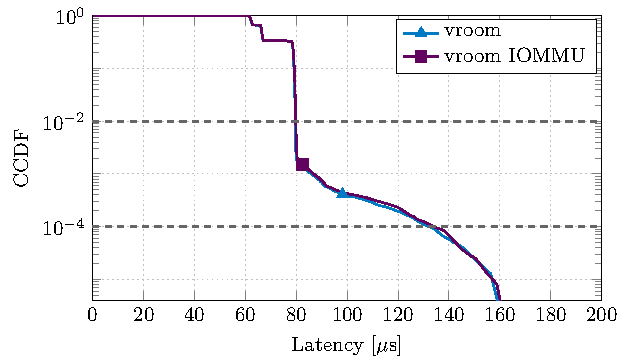
\includegraphics[width=.70\textwidth]{figures/lats_ccdf_2MiB_qd1t1_read} \label{fig:ccdf-read}}
  \subcaptionbox {Random write} {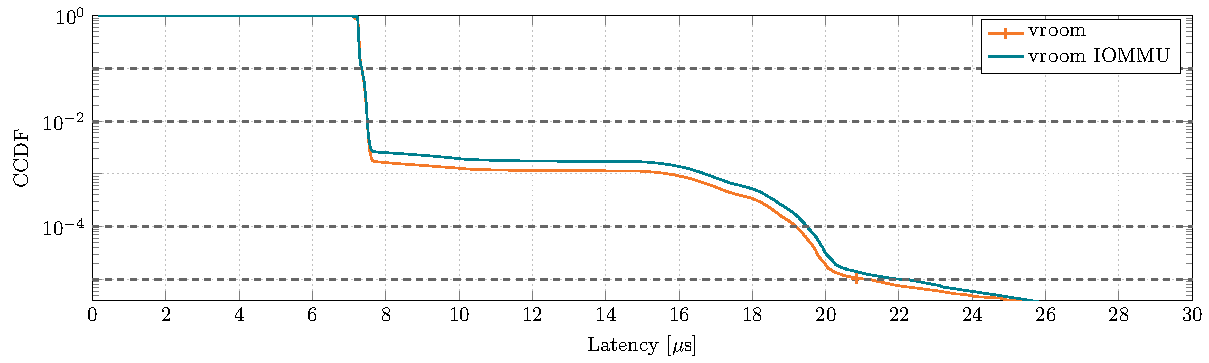
\includegraphics[width=.70\textwidth]{figures/lats_ccdf_2MiB_qd1t1} \label{fig:ccdf-write}}
  \caption{Tail latencies (60s) on Intel System}
  \label{fig:ccdf}
\end{figure}

\begin{figure}[H]
  \centering
  \subcaptionbox {Random read} {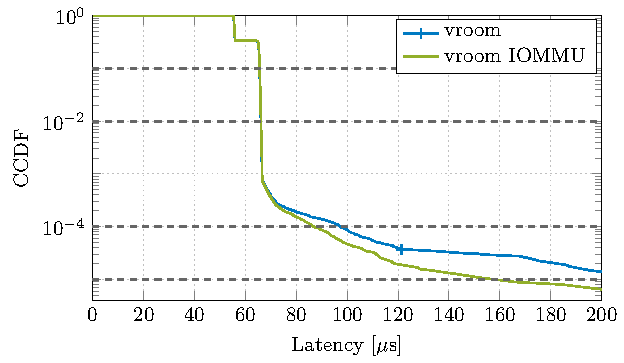
\includegraphics[width=.70\textwidth]{figures/lats_ccdf_2MiB_qd1t1_read_epyc} \label{fig:ccdf-read-epyc}}
  \subcaptionbox {Random write} {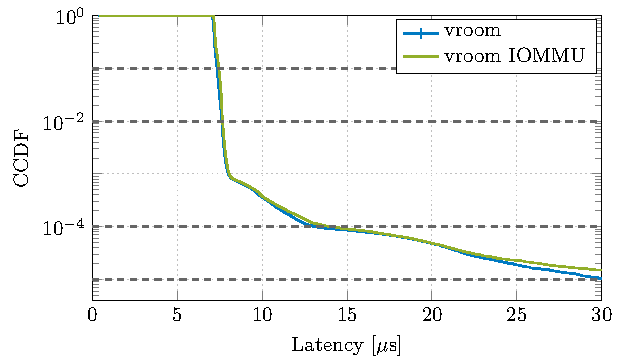
\includegraphics[width=.70\textwidth]{figures/lats_ccdf_2MiB_qd1t1_epyc} \label{fig:ccdf-write-epyc}}
  \caption{Tail latencies (60s) on AMD System}
  \label{fig:ccdf-epyc}
\end{figure}

\autoref{fig:ccdf} and \autoref{fig:ccdf-epyc} show that the latency distribution is the same with IOMMU as without. The lines are mostly overlapping. This shows that there are no significant latency spikes that occur due to the IOMMU.

\subsection{Throughput}
To test the overall throughput we perform random reads/writes over 60 seconds once with singlethreaded I/O and queue depth 1 and once with queue depth 32 and 4 threads. As seen on \autoref{fig:throughput-bar}, the IOMMU has no noticeable performance impact. Even with the higher queue depth and thread count, the performance is identical.

\begin{figure}[H]
  \centering
  \subcaptionbox {Queue depth 1 and 1 thread} {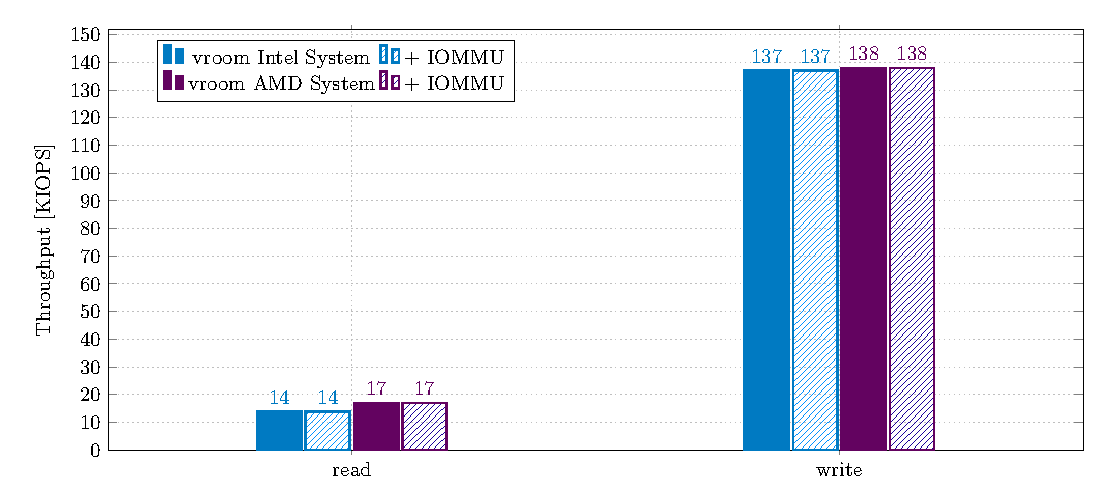
\includegraphics[width=.9\textwidth]{figures/throughput_bar_qd1t1} \label{fig:throughput-qd1t1}}
  \subcaptionbox {Queue depth 32 and 4 threads} {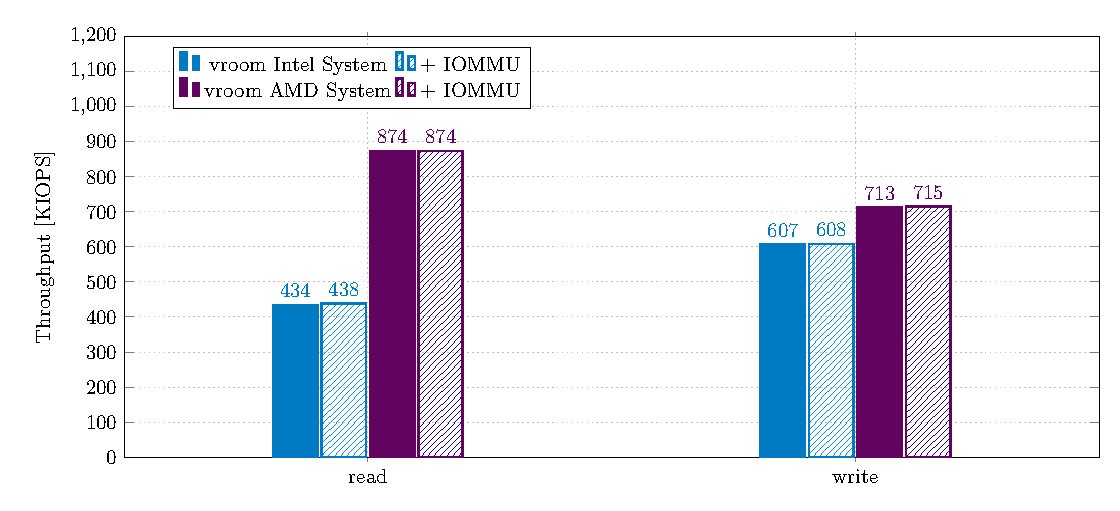
\includegraphics[width=.9\textwidth]{figures/throughput_bar_qd32t4} \label{fig:throughput-qd32t4}}
  \caption{Throughput of singlethreaded and multithreaded I/O over 60s}
  \label{fig:throughput-bar}
\end{figure}

We also take a look at throughput performance with larger queue depths. The performance is mostly the same, but a slight performance difference is noticeable on the AMD system, where the maximum throughput of vroom with IOMMU is around 3\% higher than without the IOMMU.

\begin{figure}[H]
  \centering
  \subcaptionbox {Intel System} {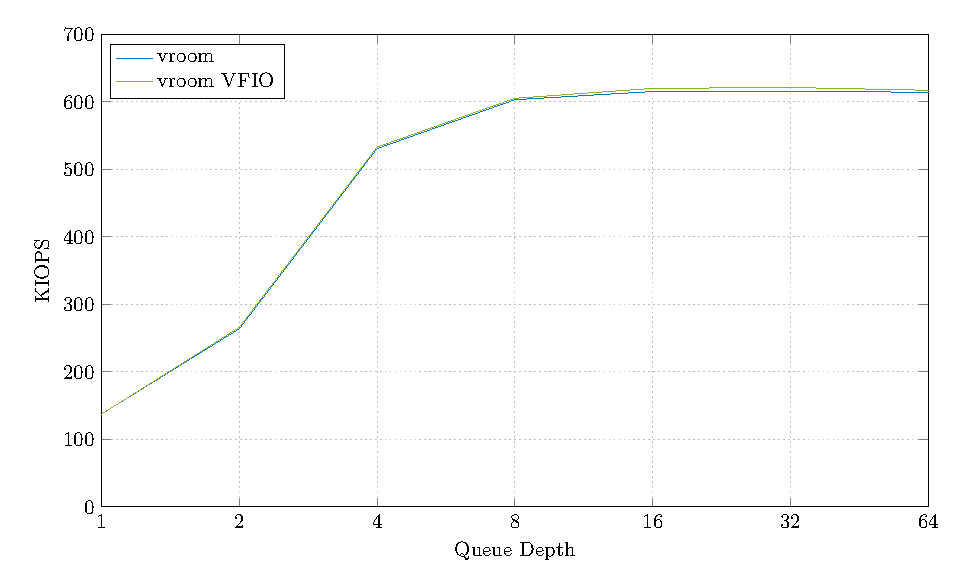
\includegraphics[width=.8\textwidth]{figures/qdnt1_2MiB} \label{fig:qdnt1-2MiB-intel}}
  \subcaptionbox {AMD System} {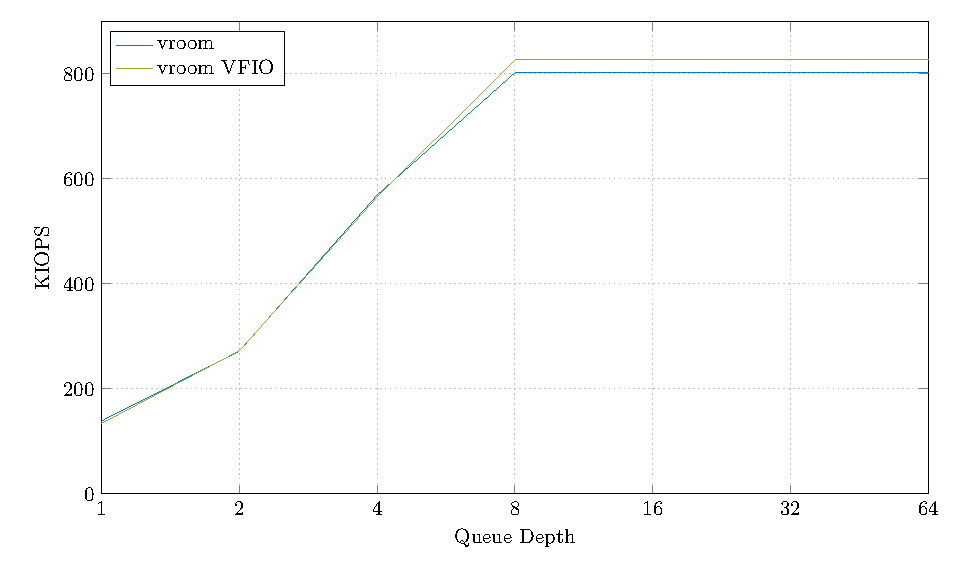
\includegraphics[width=.8\textwidth]{figures/qdnt1_2MiB_epyc} \label{fig:qdnt1-2MiB-epyc}}
  \caption{Random write throughput with increasing Queue Depth over 60s}
  \label{fig:qdnt1-2MiB}
\end{figure}

\paragraph{Using multiple SSDs} We further push the throughput by using 8 NVMes with high queue depth and thread counts in parallel in \autoref{fig:throughput-bar-8n}. Again, no significant performance impact occurs. Each NVMe has a slightly higher throughput than when tested alone.

\begin{figure}[H]
  \centering
  \subcaptionbox {Queue depth 1 and 1 thread\label{fig:throughput-qd1t1-8n}} {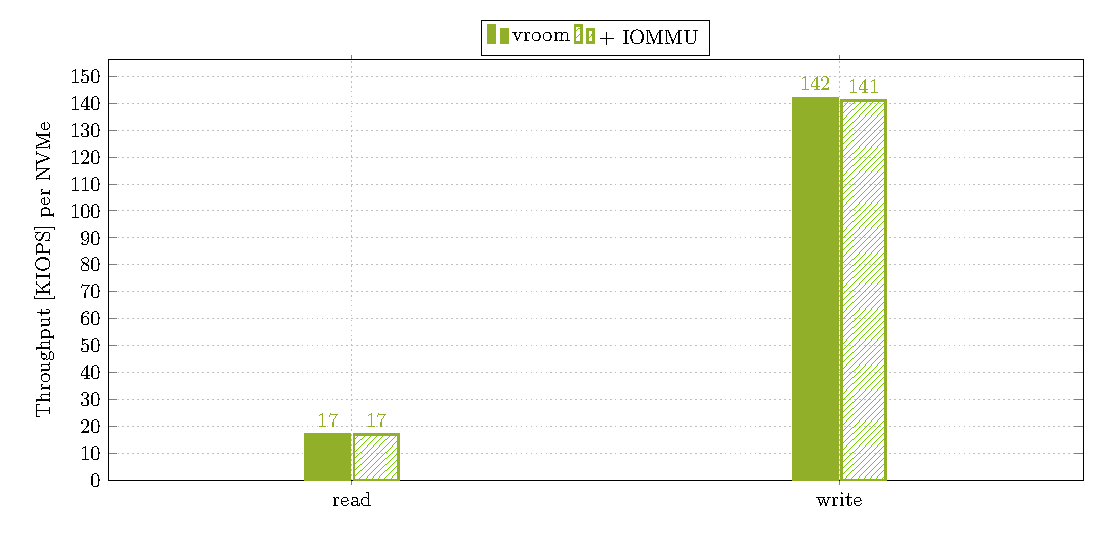
\includegraphics[width=.7\textwidth]{figures/throughput_bar_qd1t1_8nvmes} }
  \subcaptionbox {Queue depth 32 and 4 threads\label{fig:throughput-qd32t4-8n}} {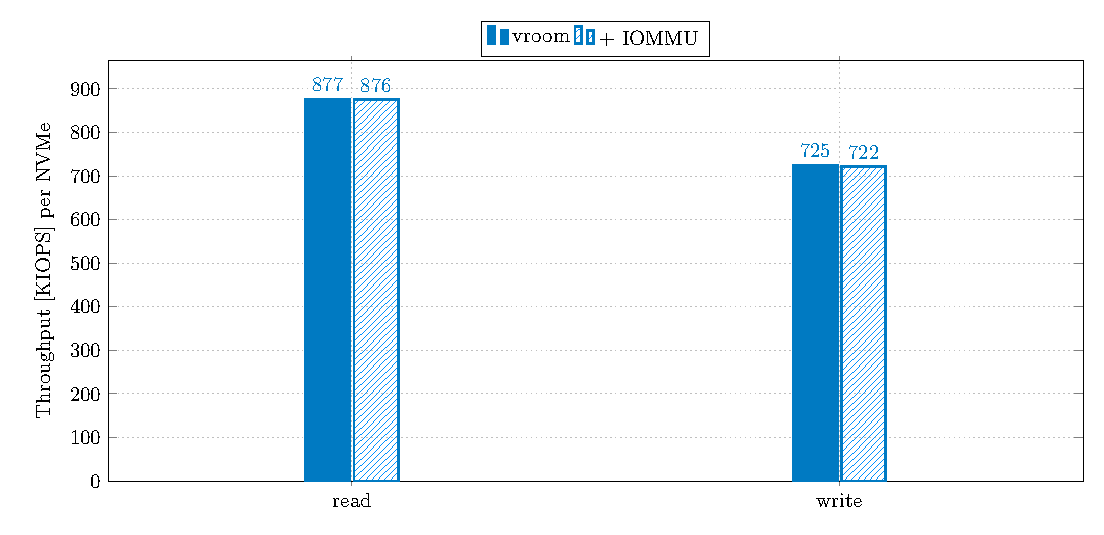
\includegraphics[width=.7\textwidth]{figures/throughput_bar_qd32t4_8nvmes} }
  \subcaptionbox {Queue depth 128 and 16 threads\label{fig:throughput-qd128t16-8n}} {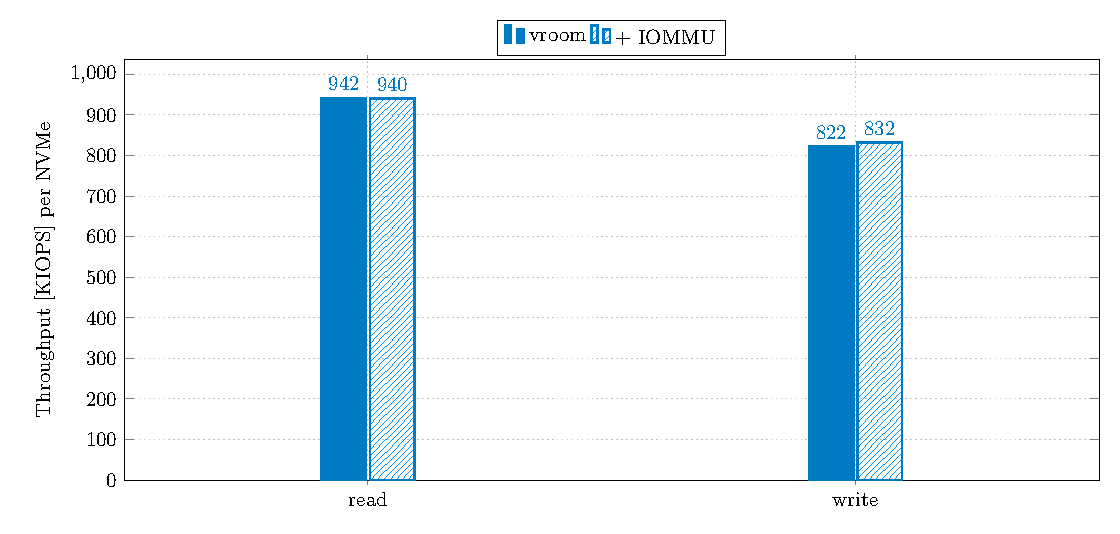
\includegraphics[width=.7\textwidth]{figures/throughput_bar_qd128t16_8nvmes} }
  \caption{Throughput over 60s on 8 NVMe SSDs on the AMD system}
  \label{fig:throughput-bar-8n}
\end{figure}

\section{Impact of \qty{4}{\kibi\byte} pages}
\subsection{Throughput}
As Linux, as well as our IOMMUs, support \qty{4}{\kibi\byte}, \qty{2}{\mebi\byte} and \qty{1}{\gibi\byte} page sizes, we will test and analyze how it affects the latencies and overall performance. A performance impact should be noticeable, especially using \qty{4}{\kibi\byte} pages. As we use a typical unit size of \qty{4}{\kibi\byte}, using \qty{4}{\kibi\byte} pages should result in TLB-thrashing, i.e., every I/O operation resulting in a page walk. To test this hypothesis, we focus on the Intel system and only write to the Turbowrite buffer of the Samsung Evo 970 Plus to reach the maximum performance and lowest latencies. We test this using an increasing number of threads in \autoref{fig:qd1tn-4kib} and an increasing queue depth in \autoref{fig:qdnt1-4kib}.

\begin{figure}[H]
  \centering
  \subcaptionbox {1 \qty{4}{\kibi\byte} buffer per thread} {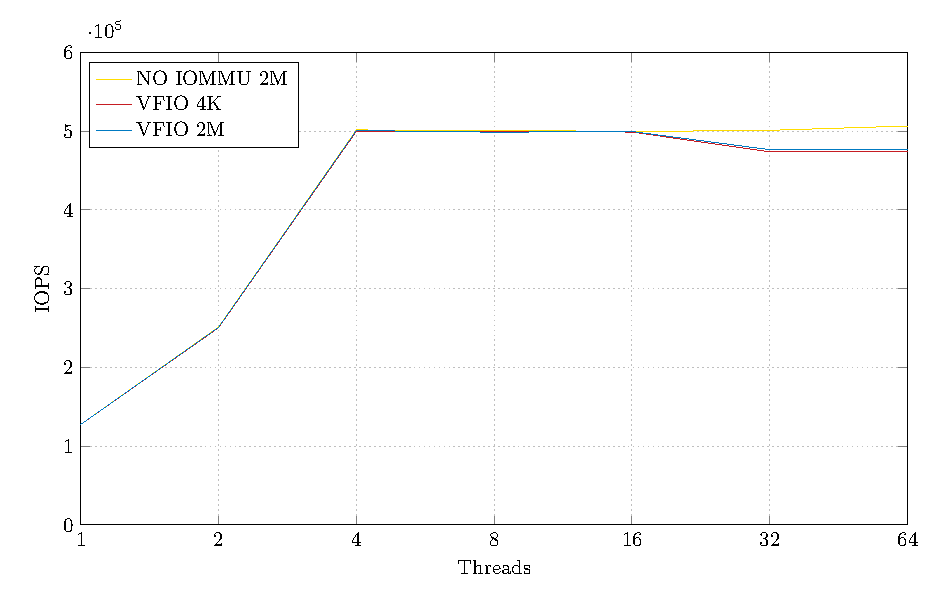
\includegraphics[width=0.6\textwidth]{figures/qd1tn_1page}}
  \subcaptionbox {1 \qty{2}{\mebi\byte} buffer per thread} {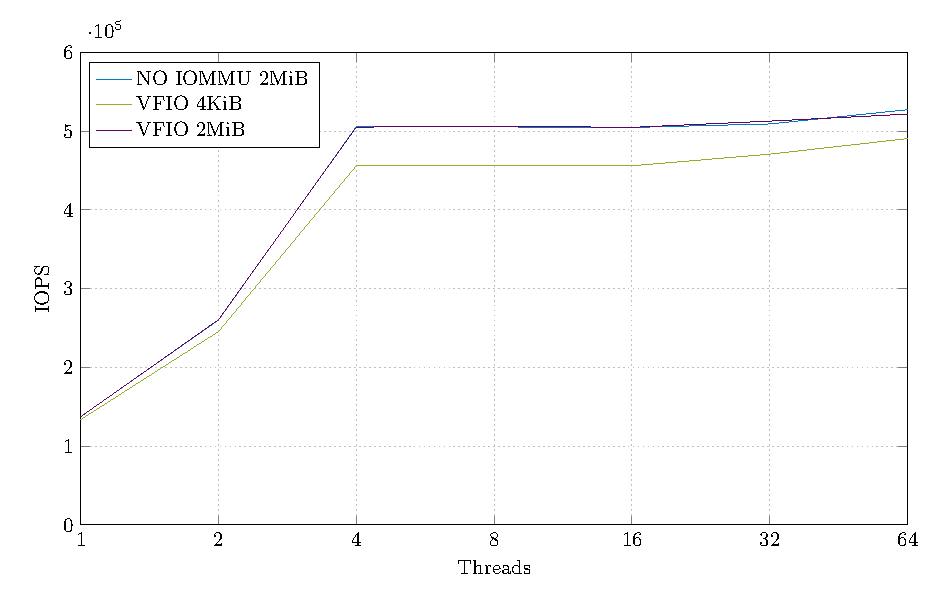
\includegraphics[width=0.6\textwidth]{figures/qd1tn_512page}}
  \caption{Random write throughput over 20s with increasing thread count and queue depth 1 on the Intel system}
  \label{fig:qd1tn-4kib}
\end{figure}

In \autoref{fig:qd1tn-4kib}, when comparing the performance of vroom without the IOMMU against vroom with IOMMU using \qty{4}{\kibi\byte} and \qty{2}{\mebi\byte} pages on a 2MiB buffer, a performance difference of around 10\% between \qty{4}{\kibi\byte} pages and \qty{2}{\mebi\byte} pages can be observed. This stems from the aforementioned IOTLB-thrashing. Noticeable is that no performance impact can be seen when using a 4KiB buffer, as all pages can fit into the IOTLB. The lines of both implementations using \qty{2}{\mebi\byte} pages overlap with both buffer sizes.

\begin{figure}[H]
  \centering
  \subcaptionbox {1 \qty{4}{\kibi\byte} buffer per thread} {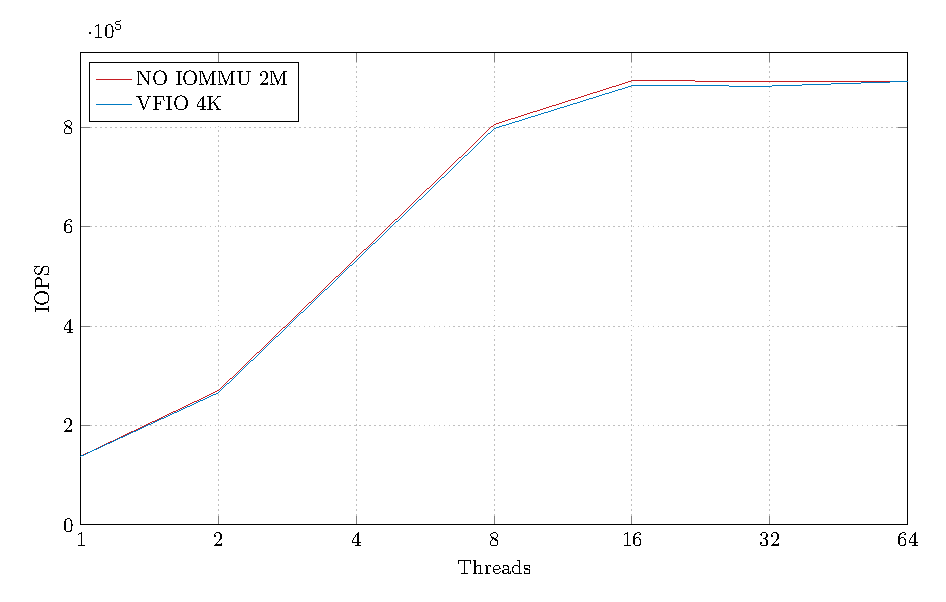
\includegraphics[width=0.6\textwidth]{figures/qdnt1_1page}}
  \subcaptionbox {1 \qty{2}{\mebi\byte} buffer per thread} {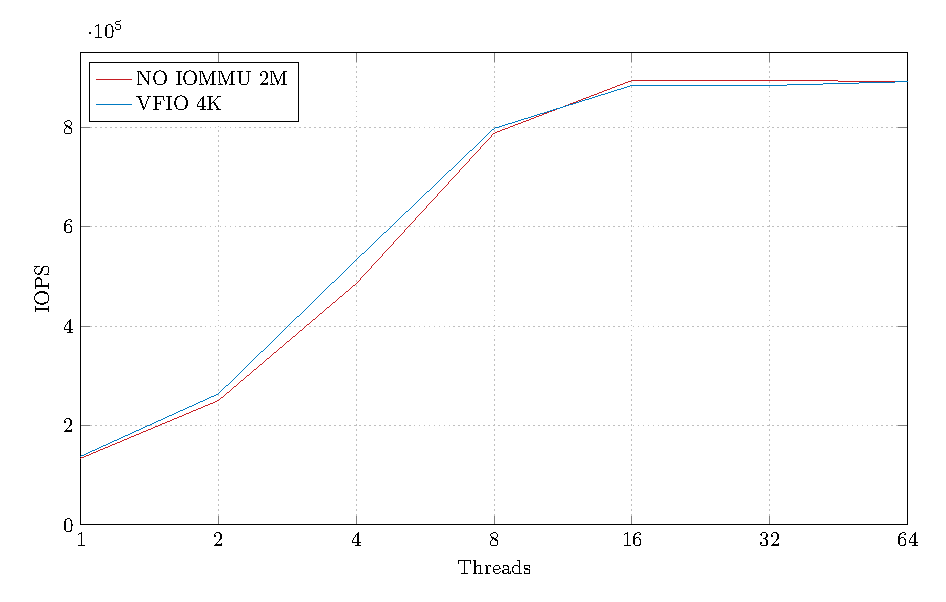
\includegraphics[width=0.6\textwidth]{figures/qdnt1_512page}}
  \caption{Singlethreaded random write throughput over 20s with increasing queue depth on the Intel system}
  \label{fig:qdnt1-4kib}
\end{figure}

In \autoref{fig:qdnt1-4kib}, a 10\% performance decrease can be seen at queue depth 4. This difference grows smaller as we further increase the queue depth, though. At 16 or more queue depth the throughput caps at around 890KIOPS, and no more substantial difference between the implementations can be measured. As we have seen a constant decrease of 10\% in performance when testing multiple threads in \autoref{fig:qd1tn-4kib}, we suspect that the PCIe bus is the bottleneck and limiting the performance.

\paragraph{PCIe limitations}
The Intel System SSD is mounted on a PCIe 3.0 4x width bus with a maximum payload of 256 bytes. This PCI bus has a maximum throughput of 3.938 GB/s. Using the SSD to its full capability, i.e. using random writes with high queue depths in the Turbowrite buffer, can result in the bus being the bottleneck. With the highest throughput measured being 890K IOPS with one I/O operation containing 4096 bytes of data, we achieve 3.64 GB/s. Including the headers for each TLP and submission- and completion queue entries, we come to a result of 3.908 GB/s. This roughly equates the PCIe bus limit and leads us to conclude, that the missing overhead of using \qty{4}{\kibi\byte} pages on high queue depths stems from this bottleneck.

\subsection{Determining IOTLB size}
As the size of the IOTLB is not stated in hardware and VT-d or AMD-V specifications, we use a latency test to analyze the behaviour of the IOMMU.
In order to isolate the effect of the IOMMU we track the latencies of the fastest operation the NVMe can perform. The lowest latency is achieved by carrying out a random write using the smallest block size of \qty{512}{\byte}.

If we then write from a single block from each page to the NVMe, repeat it 65536 times on an increasing page count that are a power of two, we can figure out where a latency spike occurs. The page count right before the latency spike should equal the IOTLB entry count. We configure the queues, buffer and prp-list to each take up one page, resulting in a maximum of 6 pages in the IOTLB before the actual workload.
The test is performed with VFIO with \qty{4}{\kibi\byte}, \qty{2}{\mebi\byte} and \qty{1}{\gibi\byte} pages and without the IOMMU with \qty{2}{\mebi\byte} pages as reference. As we have limited available memory, the \qty{1}{\gibi\byte} pages could only be tested to 112 pages on the Intel system and 128 on the AMD system.

\begin{figure}[H]
  \centering
  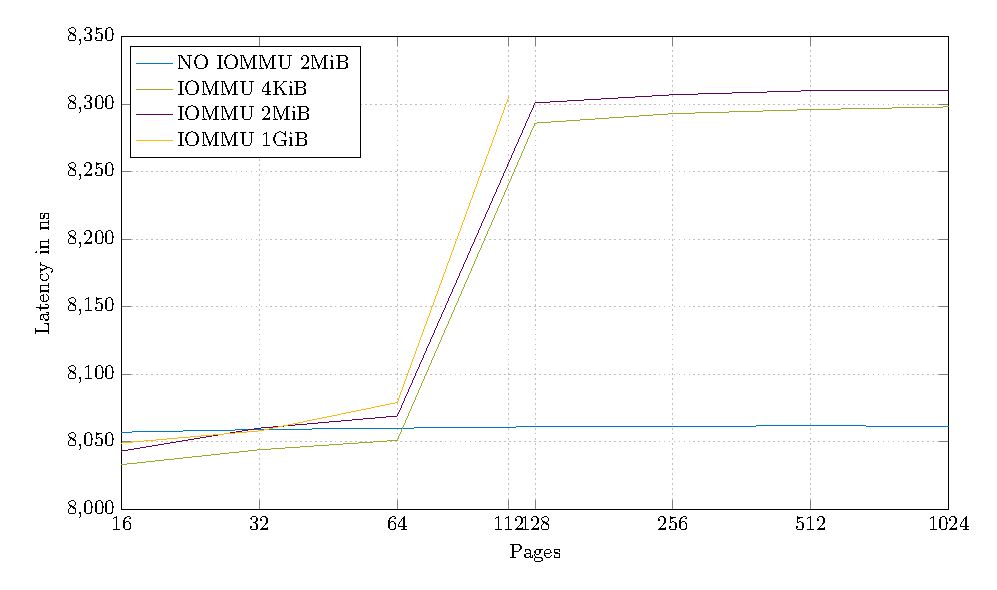
\includegraphics[width=\textwidth]{figures/psmeds}
  \caption{Latencies of random writes on an emptied SSD with increasing pages in memory on the Intel system}
  \label{fig:med-ps}
\end{figure}

\paragraph{Results of Intel Xeon E5-2660v2}
In the resulting graph \autoref{fig:med-ps} we can observe a performance spike of around 250 nanoseconds for each write between 64 and 128 allocated pages. In the case of \qty{4}{\kibi\byte} pages, this is a memory size of only 512 KiB. Using this information, we can assume that the IOTLB has the same size for each pagesize, as well as it \textbf{being 64 entries of size}. This matches the page size Stefan Huber and Rolf Neugebauer found \cite{iommuhuber}\cite{pcieperfnegebauer}.

\begin{figure}[H]
  \centering
  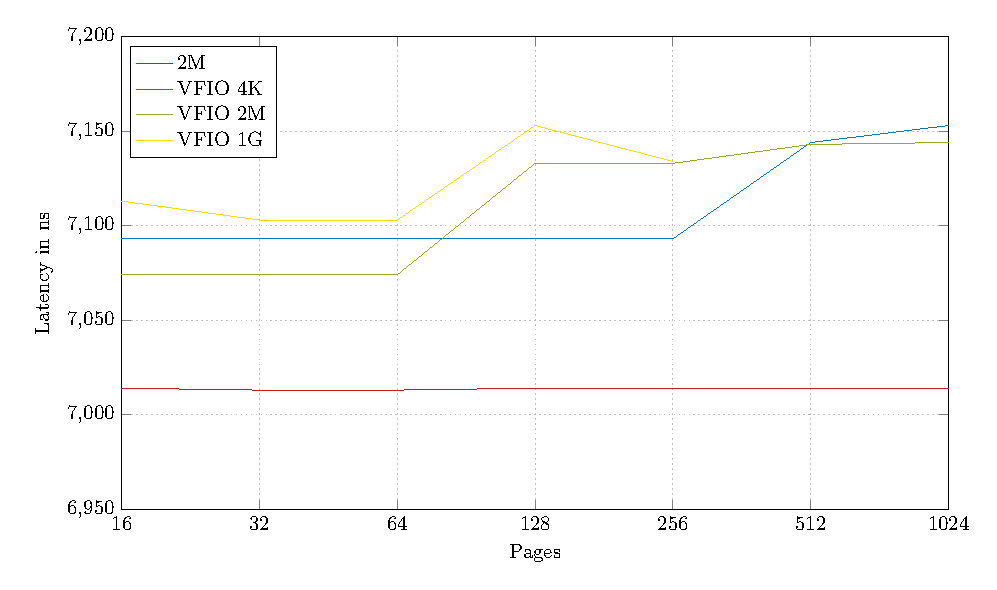
\includegraphics[width=\textwidth]{figures/psmedsepyc}
  \caption{Latencies of random writes on an emptied SSD with increasing pages in memory on the AMD system}
  \label{fig:med-psepyc}
\end{figure}

\paragraph{Results of AMD EPYC 7713}
On the AMD IOMMU, we can see three performance spikes. Each occurs between 32-64 pages for \qty{1}{\gibi\byte} pages, 64-128 pages for \qty{2}{\mebi\byte}, and 256-512 for \qty{4}{\kibi\byte} pages.
We can therefore assume that the IOTLB size depends on the pagesize unlike on the Intel CPU. This leads us to suspect an \textbf{IOTLB size of 32 for \qty{1}{\gibi\byte} pages, 64 for \qty{2}{\mebi\byte} pages and 256 for \qty{4}{\kibi\byte} pages}. The latencies only decrease by about \qty{60}{ns}, which is a about four times less than page walks on the Intel system.